\documentclass[a4paper,11pt,twocolumn]{article}
\usepackage[latin1]{inputenc}
\usepackage[english]{babel}
\usepackage{amsmath}
\usepackage{amsfonts}
\usepackage{amssymb}
\usepackage{mathtools}
\usepackage{cancel}

\usepackage{titling}
\usepackage{nomencl}
\usepackage{siunitx}
\usepackage[style=ieee,backend=bibtex]{biblatex}
\usepackage[font={small}]{caption}
\usepackage{subcaption}

\usepackage{graphicx}
\usepackage{color}

\usepackage{float}
\usepackage{afterpage}

\usepackage{booktabs}
\usepackage{threeparttable}
\usepackage{multirow}
\usepackage{calc}
\usepackage{fancyhdr}

\usepackage{textcomp}
\usepackage{varioref}
\usepackage{xspace}
\usepackage[activate={true,nocompatibility},final,tracking=true,kerning=true,spacing=nonfrench,factor=1100,stretch=10,shrink=10]{microtype}
% activate={true,nocompatibility} - activate protrusion and expansion final -
% enable microtype; use "draft" to disable tracking=true, kerning=true,
% spacing=true - activate these techniques factor=1100 - add 10% to the
% protrusion amount (default is 1000) stretch=10, shrink=10 - reduce
% stretchability/shrinkability (default is 20/20) Reduce tracking around small
% caps to 40%
\SetTracking{encoding={*}, shape=sc}{40}

% Document info.
\author{Z0966990}
\title{M23 Lab Report}
\date{\today}

% Path to images.
\graphicspath{{img/}}

% Setup nomenclature.
\newlength{\nomtitlesep}
\setlength{\nomtitlesep}{\nomitemsep}
\setlength{\nomitemsep}{-0.8\parsep}
\renewcommand\nomgroup[1]{
    \ifthenelse{\equal{#1}{A}}{
        \itemsep\nomtitlesep
        \item[\textbf{Acronyms}]
        \itemsep\nomitemsep}{
    \ifthenelse{\equal{#1}{B}}{
        \itemsep\nomtitlesep
        \item[\textbf{Background}]
        \itemsep\nomitemsep}{
    \ifthenelse{\equal{#1}{C}}{
        \itemsep\nomtitlesep
        \item[\textbf{Experiment}]
        \itemsep\nomitemsep}{
    %else
        \itemsep\nomtitlesep
        \item[\textbf{\textcolor{red}{Undefined}}]
        \itemsep\nomitemsep
}}}}
\makenomenclature

% Setup bibiliography.
\addbibresource{m23_lab_report.bib}

% Header and footer.
\pagestyle{fancy}
\fancyhf{}
\lhead{\thetitle}
\rhead{\theauthor}
\cfoot{\thepage}
\renewcommand{\headrulewidth}{0pt}
\renewcommand{\footrulewidth}{0pt}

% Macros.
\newcommand{\CSA}{\textsc{CSA}\xspace}
\newcommand{\BEM}{\textsc{BEM}\xspace}
\newcommand{\SE}{\textsc{SE}\xspace}

\newcommand{\GPa}{\si{\giga\pascal}\xspace}
\newcommand{\MPa}{\si{\mega\pascal}\xspace}
\newcommand{\mm}{\si{\milli\meter}\xspace}

\begin{document}
    
% Title page.
\begin{titlepage}
    \centering
    \vspace*{\fill}
    
\includegraphics[width=0.5\textwidth]{Durham.png}\\
    \vspace*{\fill}
    \LARGE\thetitle\\
    \large\theauthor\\
    \large L2 Mechanical Engineering\\
    \large\thedate\\
    \vspace*{\fill}
\end{titlepage}

% Main matter.
\renewcommand{\abstractname}{\large Abstract}
\twocolumn[
\begin{@twocolumnfalse}
    \begin{abstract}
        In this report it is detailed how empirical, numerical and analytical
        approaches were used to investigate how stress and strain concentrations
        in plates vary around features. Strain gauges were used to measure the
        deformation of a plate under axial load with a circular hole stress
        raiser at the centre. From those measurements, the strain and stress
        concentrations in the plate were deduced. Those concentrations were
        compared to concentrations predicted by numerical simulations and
        analytical expressions. Numerical simulations were used to explore the 
        relationship between the dimensions of shoulder fillets and the stress 
        concentrations surrounding them. Parallels were then drawn between the
        circular hole and shoulder fillet stress raisers.
    \end{abstract}
\end{@twocolumnfalse}
\vspace{\parsep}
]

% Acronyms
% \nomenclature[A0]{\CSA}{Computational stress analysis}
\nomenclature[A1]{\BEM}{Boundary element method}
\nomenclature[A2]{\SE}{Standard error}
\nomenclature[AA]{~}{\vspace*{-\baselineskip}}

% Theory
\nomenclature[B00]{$E$}{Young's modulus of elasticity
    \hspace*{\fill}\GPa}
\nomenclature[B01]{$H$}{Height of plate
    \hspace*{\fill}\mm}
\nomenclature[B02]{$K_\epsilon$}{True strain concentration factor
    \hspace*{\fill}---}
% \nomenclature[B03]{$K_{\epsilon_t}$}{Theoretical strain concentration factor\\
%     \hspace*{\fill}---}
\nomenclature[B04]{$K_\sigma$}{True stress concentration factor
    \hspace*{\fill}---}
\nomenclature[B05]{$K_{\sigma_t}$}{Theoretical stress concentration factor\\
    \hspace*{\fill}---}
\nomenclature[B06]{$L$}{Length of plate
    \hspace*{\fill}\mm}
\nomenclature[B07]{$S$}{Far-field stress
    \hspace*{\fill}\MPa}
\nomenclature[B08]{$d$}{Height/diameter of plate feature
    \hspace*{\fill}\mm}
\nomenclature[B09]{$r$}{Radius of plate feature
    \hspace*{\fill}\mm}
% \nomenclature[B10]{$\gamma_{uv}$}{Shear strain in $uv$-plane
%     \hspace*{\fill}---}
\nomenclature[B11]{$\epsilon_{nom}$}{Nominal strain
    \hspace*{\fill}---}
\nomenclature[B12]{$\epsilon_{ww}$}{Normal strain in $w$-direction
    \hspace*{\fill}---}
\nomenclature[B13]{$\nu$}{Poisson's ratio
    \hspace*{\fill}---}
\nomenclature[B14]{$\sigma_{max}$}{Maximum plate stress
    \hspace*{\fill}\MPa}
\nomenclature[B15]{$\sigma_{nom}$}{Nominal stress
    \hspace*{\fill}\MPa}
\nomenclature[B16]{$\sigma_{ww}$}{Normal stress in $w$-direction
    \hspace*{\fill}\MPa}
% \nomenclature[B17]{$\sigma_{uv}$}{Shear stress in $uv$-plane
%     \hspace*{\fill}\MPa}
\nomenclature[BB]{}{\vspace{-\baselineskip}}

% Experiment
\nomenclature[C0]{$R^2$}{Coefficient of determinability
    \hspace*{\fill}---}
\nomenclature[C1]{$K_{\epsilon_i}$}{Strain concentration factor at gauge $i$\\
    \hspace*{\fill}---}
\nomenclature[C2]{$K_{\sigma_i}$}{Stress concentration factor at gauge $i$\\
    \hspace*{\fill}---}
\nomenclature[C3]{$\Delta$}{Gradient
    \hspace*{\fill}---}
\nomenclature[C4]{$\alpha,\beta$}{Regression coefficients
    \hspace*{\fill}---}
\nomenclature[C5]{$\epsilon_i$}{Strain at gauge $i$
    \hspace*{\fill}---}
\nomenclature[C6]{$\sigma_i$}{Stress at gauge $i$
    \hspace*{\fill}\MPa}
\nomenclature[CC]{}{\vspace{-\baselineskip}}

\printnomenclature

\section{Introduction}

When designing structural components, engineers typically look to the most
stressed point in that component to determine and specify failure criteria and
factors of safety.

In simple systems, engineers can use intuition to identify candidates for
possible points of failure. In more complex systems, such as components
with smoothly varying features, more rigorous approaches to stress analysis 
are required. Experimentation, simulation and theory can all identify the most 
severely stressed point in a component.

In this report, finite width plates with either circular holes or shoulder
fillets were analysed. Circular holes are a common feature present in many
parts, allowing for fixtures such as screws and bolts to be used. Shoulder
fillets are introduced to reduce the peak stress experienced by components with
sharp internal corners.

\section{Background}

Plane stress problems are defined by their zero out of plane stress. The most 
common plane stress situations involve stresses resolved on the surface of 
plates.

On the plate boundary, the only non-zero principle stress component is
tangential to the plate boundary. The relationship between the tangential 
stress and strain can be described using Hooke's law under axial load, given 
by \mbox{Hibbeler~\cite[p.~88]{hibbeler2017mechanics}}:
\begin{equation} \label{eq:hooke-axial}
    \sigma_{xx} = E\epsilon_{xx}
\end{equation}
where $x$ is the axial or tangential direction.

In the axial load case, shear strain is also zero. The Poisson
effect can be used to determine Poisson's ratio if the axial and
transverse strains are known. The following expression was also given by
\mbox{Hibbler~\cite[p.~106]{hibbeler2017mechanics}}:
\begin{equation} \label{eq:poisson}
    \nu = -\frac{\epsilon_{yy}}{\epsilon_{xx}} 
        = -\frac{\epsilon_{zz}}{\epsilon_{xx}}
\end{equation}

\subsection{Stress Concentrations} \label{sec:stress-conc}

The stress concentration factor is a dimensionless quantity which describes how
much greater the maximum principle stress in the feature is than the 
nominal---or  average---stress in the part. Similarly, there also exists a 
strain concentration factor, which is a measure of relative deformation.
According to \mbox{Pilkey~\cite[p.~4]{pilkey2008peterson}}:
\begin{align}
    \label{eq:stress-conc}
    K_\sigma &= \frac{\sigma_{max}}{\sigma_{nom}} \\
    \label{eq:strain-conc}
    K_\epsilon &= \frac{\epsilon_{max}}{\epsilon_{nom}}
\end{align}

For simple features---or stress raisers---such as the 
circular hole in Figure~\vref{fig:hole-contour}, the \emph{theoretical} stress
concentration factor $K_{\sigma_t}$ can be determined analytically as described
by \mbox{Pilkey~\cite[pp.~180--181]{pilkey2008peterson}}:
\begin{equation} \label{eq:inf-hole-conc}
    K_{\sigma_t} = 3
\end{equation}

\begin{figure}[h]
    \centering
    \def\svgwidth{\linewidth}
    \input{img/hole_conc.pdf_tex}
    \caption{Circular hole stress concentrations.}
    \label{fig:hole-contour}
\end{figure}

Pilkey also offers equations to determine the local stress concentrations at
any point in the plate; used to produce the contour plot in 
Figure~\ref{fig:hole-contour}. These reveal most stressed---red---points lie
at the top and bottom of the hole.

However, when the plate has a finite width as illustrated in 
Figure~\vref{fig:hole-dims}, the problem becomes much harder to solve
analytically. Howland~\cite{howland1930stresses} derived a more generalised 
stress concentration factor expression at the top and bottom of the hole, but
not for the local stress concentrations throughout the rest of the plate:
\begin{equation} \label{eq:hole-conc}
    K_{\sigma_t} = \frac{2 + (1 - d/H)^3}{1 - d/H}
\end{equation}

\begin{figure}[h]
    \centering
    \def\svgwidth{\linewidth}
    \input{img/hole_dims.pdf_tex}
    \caption{Finite width plate with circular hole.}
    \label{fig:hole-dims}
\end{figure}

Notice, in the limit as $H\rightarrow\infty$,
$\eqref{eq:hole-conc}\rightarrow\eqref{eq:inf-hole-conc}$.

For the shoulder fillets detailed in Figure~\vref{fig:shoulder-dims}, stress
concentration factors are derived empirically rather than analytically.
\mbox{Pilkey~\cite[p.~151]{pilkey2008peterson}} provides a chart relating the
ratios $H/d$ and $r/d$ to the stress concentration factor using data from
multiple sources.

\begin{figure}[h]
    \centering
    \def\svgwidth{\linewidth}
    \input{img/shoulder_dims.pdf_tex}
    \caption{Finite width plate with shoulder fillets.}
    \label{fig:shoulder-dims}
\end{figure}

Therefore, to determine the location of the most stressed points, engineers must
either measure or simulate the stress concentration factors in the plate,
particularly for complex stress raisers.

One method of simulation is the Boundary Element Method---or \BEM---a modern
computational method which divides the complex part into simpler elements using 
a mesh, resolving the stresses in each element to model the stress field.

\section{Method}

\subsection{Circular Hole Stress Raiser}

To investigate the properties of a circular hole stress raiser, strain gauges
were used to measure the stress at several locations of interest in a plate 
with a circular hole placed under axial load. Figure~\vref{fig:experiment-dims} 
details the dimensions of the plate used in the experiment.

\begin{figure}[h]
    \centering
    \def\svgwidth{\linewidth}
    \input{img/experiment_dims.pdf_tex}
    \caption{Dimensions of the experiment plate.}
    \label{fig:experiment-dims}
\end{figure}

The apparatus included the plate, fixed at one end, with a thumb screw at the 
other to allow a range of loads to be applied. Strain gauges at the 
locations labelled in Figure~\vref{fig:experiment-gauges} were connected to a 
\textsc{PC} such that the strain could be measured.

\begin{figure}[h]
    \centering
    \def\svgwidth{\linewidth}
    \input{img/experiment_gauges.pdf_tex}
    \caption{Positions of strain gauges on the experiment plate.}
    \label{fig:experiment-gauges}
\end{figure}

Gauge 2 was located away from the stress raiser, so the strain measured at gauge
2 would be close to the far-field strain. Therefore, it was taken as the nominal
strain. The independent variable was the maximum strain measured across all the
strain gauges, expected to be the strain measured at gauge 7 at the bottom of
the hole. The strains measured at the other gauges were the dependent variables.

Three repeat readings were taken for five different nominal strains: 0, 
\num{200e-6}, \num{400e-6}, \num{600e-6} and \num{800e-6}. This avoided
exceeding the \num{1000e-6} limit for the apparatus, and gave sufficient repeat
readings to determine errors.

Concept Analyst\textsuperscript{\textregistered} \BEM software was used to
simulate the local stress concentrations in the plate to supplement the
experimental results.

\subsection{Shoulder Fillet Stress Raiser}

Concept Analyst was also used to investigate how changing the geometry of a 
shoulder fillet stress raiser affected the stress concentration factor. 
Figure~\vref{fig:simulation-dims} details the the defining dimensions of the 
feature.

\begin{figure}[h]
    \centering
    \def\svgwidth{\linewidth}
    \input{img/simulation_dims.pdf_tex}
    \caption{Dimensions of plate with shoulder fillets.}
    \label{fig:simulation-dims}
\end{figure}

In practice, the plate detailed in Figure~\ref{fig:simulation-dims} was modelled
with the feature height $d$ kept constant at 100~\mm. To investigate the effects
of varying the ratio $H/d$, the simulations were run with $H$ at 110~\mm,
130~\mm and 200~\mm. For each $H$ value, $r/d$ was also varied by running the
simulations with six different feature radii in the range 5~\mm--10~\mm.

$L$ was initially chosen to be ten times greater than $H$, operating under the
assumption that this was sufficiently long such that the plate behaved as if 
the far-field stress was applied an infinite distance away from the shoulder 
fillets. This allowed an infinitely long plate to be represented by a finite
model.

The nominal far-field stress $S$ was applied to the plate using a traction of
magnitude 100~\MPa. The exact magnitude of this load was not important as
the stresses were later normalised by the chosen far-field stress to find the 
stress concentration factors.

To investigate how the stress concentration factor changes in a plate with a
finite length, $L/H$ was then reduced from 5 to 0.5, corresponding to ten 
lengths in the range 1000~\mm--50~\mm. $H$ was kept constant at 200~\mm, $d$ 
at 100~\mm and $r$ at 10~\mm.

\section{Results}

\subsection{Circular Hole Stress Raiser}

Figure~\vref{fig:experiment-results} details the strains measured at each 
gauge, plotted against the nominal strain at gauge 2.

\begin{figure}[h]
    \small
    \centering
    \def\svgwidth{\linewidth}
    \input{img/experiment_results.pdf_tex}
    \caption{Strains measured around circular hole, plotted against nominal
        strain.}
    \label{fig:experiment-results}
\end{figure}

Least squares regression lines were fitted to the data for each strain gauge,
including repeats. Taking gradients of the line for each strain gauge yielded
the local stress concentration factors in Table~\vref{tab:strain-conc}. When the
nominal strain is zero, all other strains are zero, leading to the following:
\begin{equation*}
    \Delta = \frac{\epsilon_i - 0}{\epsilon_{nom}-0}
           = \frac{\epsilon_i}{\epsilon_{nom}} = K_{\epsilon_i}
\end{equation*}

\begin{table}[h]
    \small
    \centering
    \caption{Local strain concentration factors measured around circular hole.}
    \label{tab:strain-conc}
    \begin{threeparttable}
        \begin{tabular}{
            c
            S[separate-uncertainty=true,
              table-format=-1.3,
              table-figures-uncertainty=1]
        }
            \toprule
            $K_{\epsilon_1}$ & -0.314\pm0.016 \\
            $K_{\epsilon_2}$ &  1.000\pm0.000 \\
            $K_{\epsilon_3}$ &  0.348\pm0.010 \\
            $K_{\epsilon_4}$ &  1.043\pm0.032 \\
            $K_{\epsilon_5}$ &  1.001\pm0.033 \\
            $K_{\epsilon_6}$ & -1.559\pm0.040 \\
            $K_{\epsilon_7}$ &  4.564\pm0.103 \\
            $K_{\epsilon_8}$ &  1.714\pm0.045 \\
            $K_{\epsilon_9}$ &  0.760\pm0.017 \\
            \bottomrule
        \end{tabular}
        \begin{tablenotes}
            \footnotesize   
            \item $K_{\epsilon_i}\pm95\%$ confidence
        \end{tablenotes}
    \end{threeparttable}
\end{table}

\subsection{Shoulder Fillet Stress Raiser}

The contour plots for the stress concentrations in the extremes of the shoulder
fillet geometry are displayed in Figure~\vref{fig:simulation-results-contour}.

\begin{figure*}[t]
    \centering
    \begin{subfigure}[b]{0.48\textwidth}
        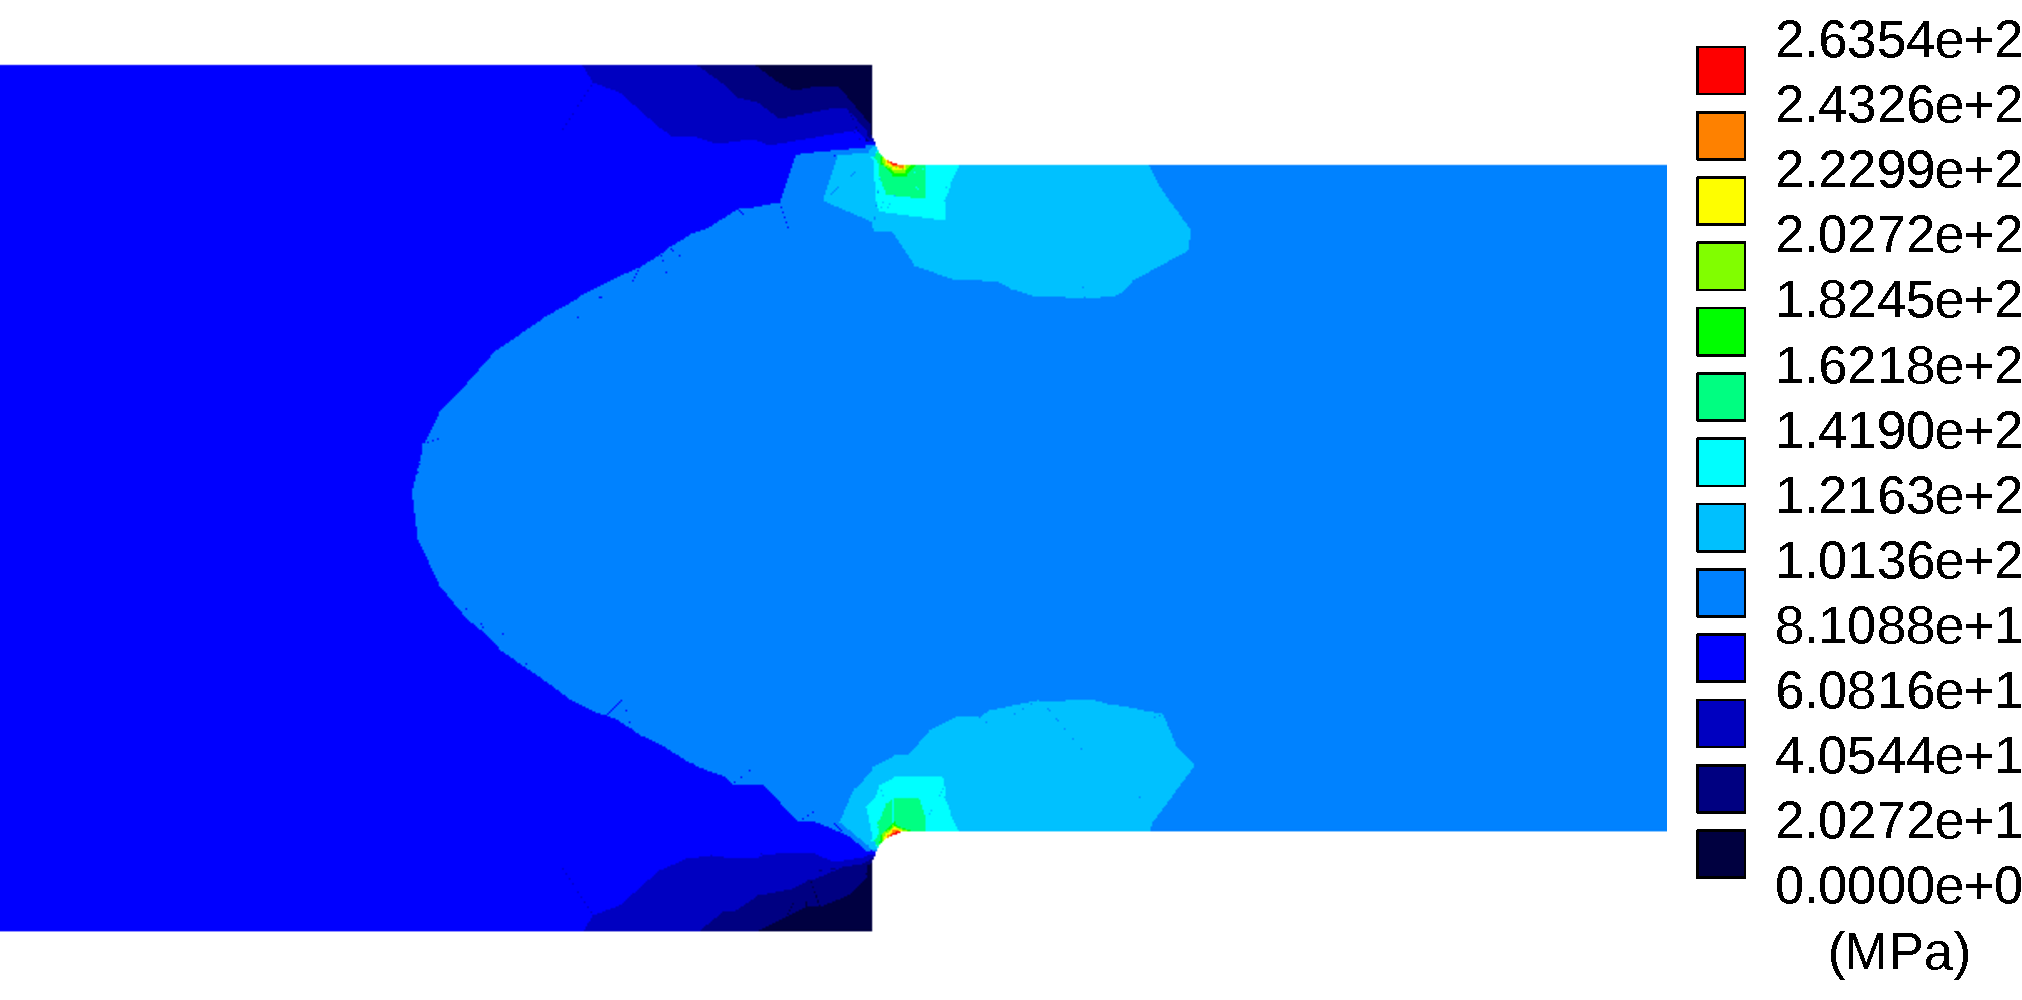
\includegraphics[width=\textwidth]{img/Hd1-3_rd0-05.pdf}
        \caption{$H/d = 1.3,r/d = 0.05$}
        \label{fig:H/d=1.3-r/d=0.05}
    \end{subfigure}
    \begin{subfigure}[b]{0.48\textwidth}
        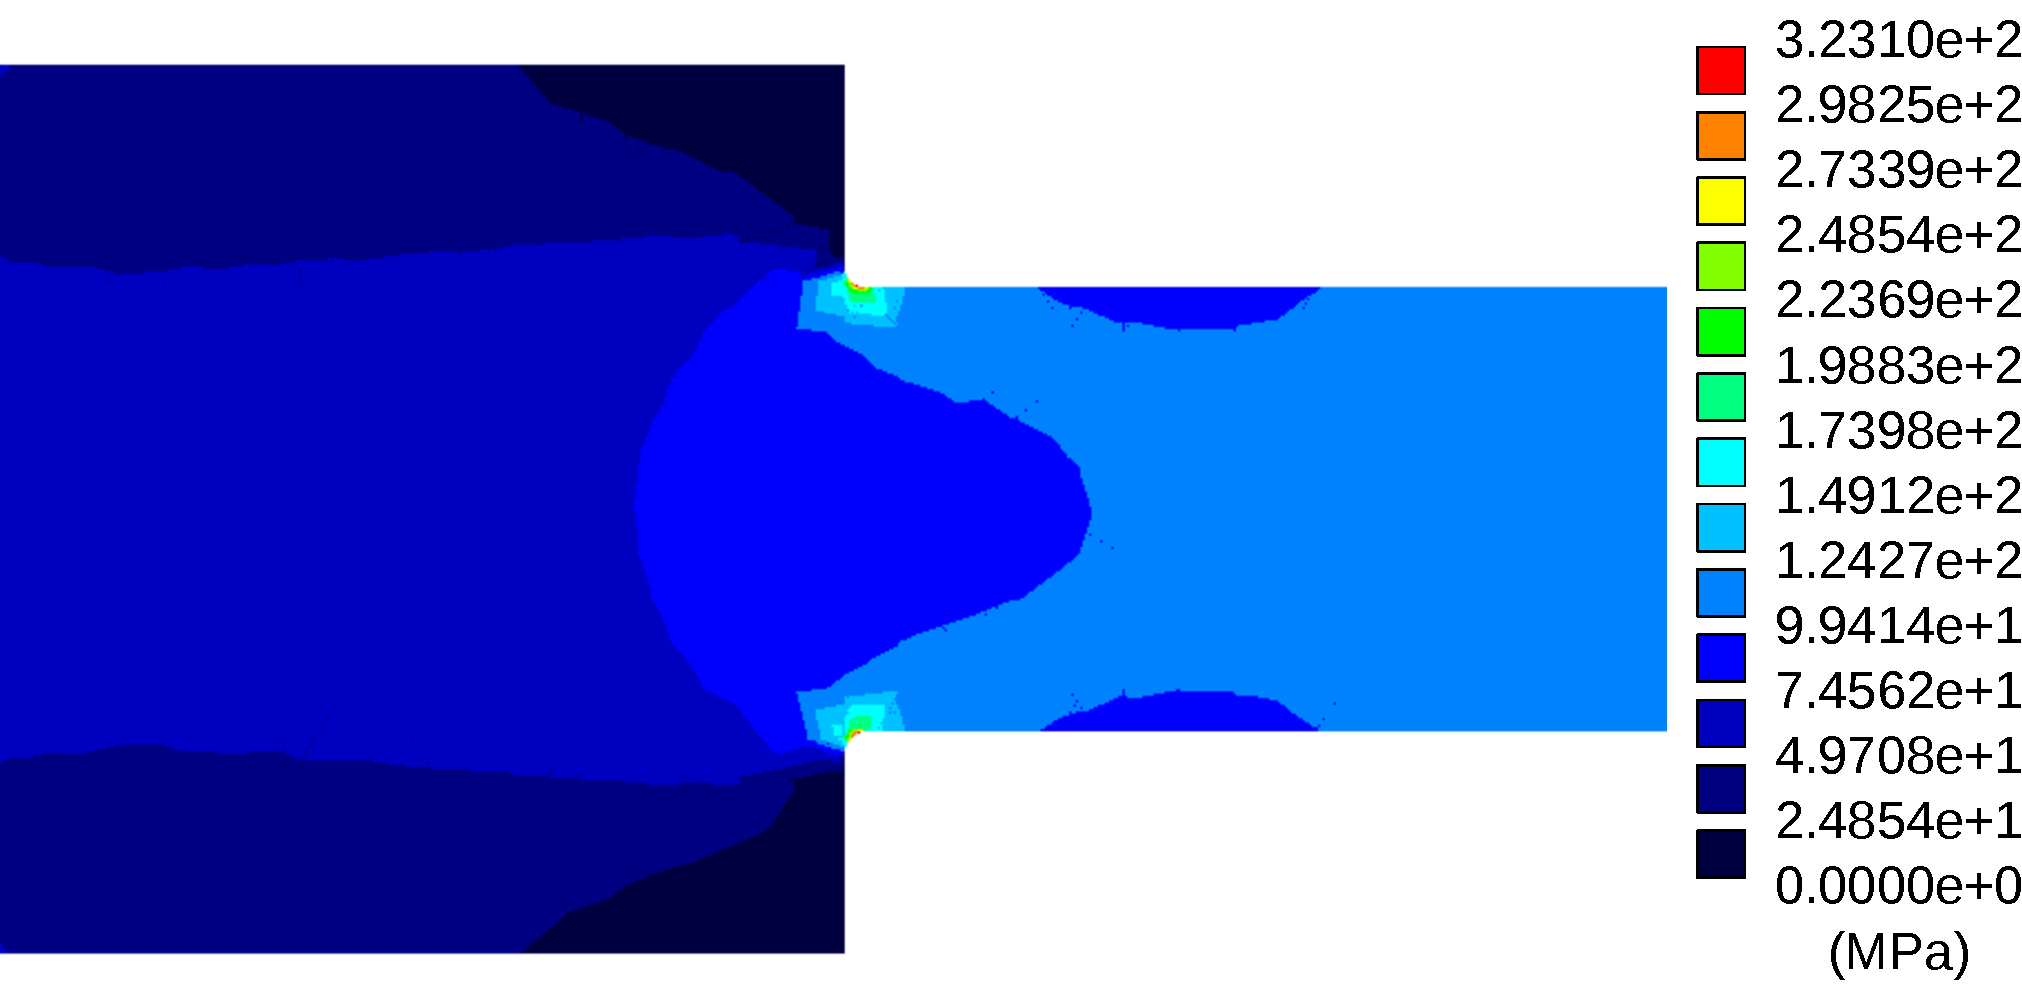
\includegraphics[width=\textwidth]{img/Hd2-0_rd0-05.pdf}
        \caption{$H/d = 2.0,r/d = 0.05$}
        \label{fig:H/d=2.0-r/d=0.05}
    \end{subfigure}
    \begin{subfigure}[b]{0.48\textwidth}
        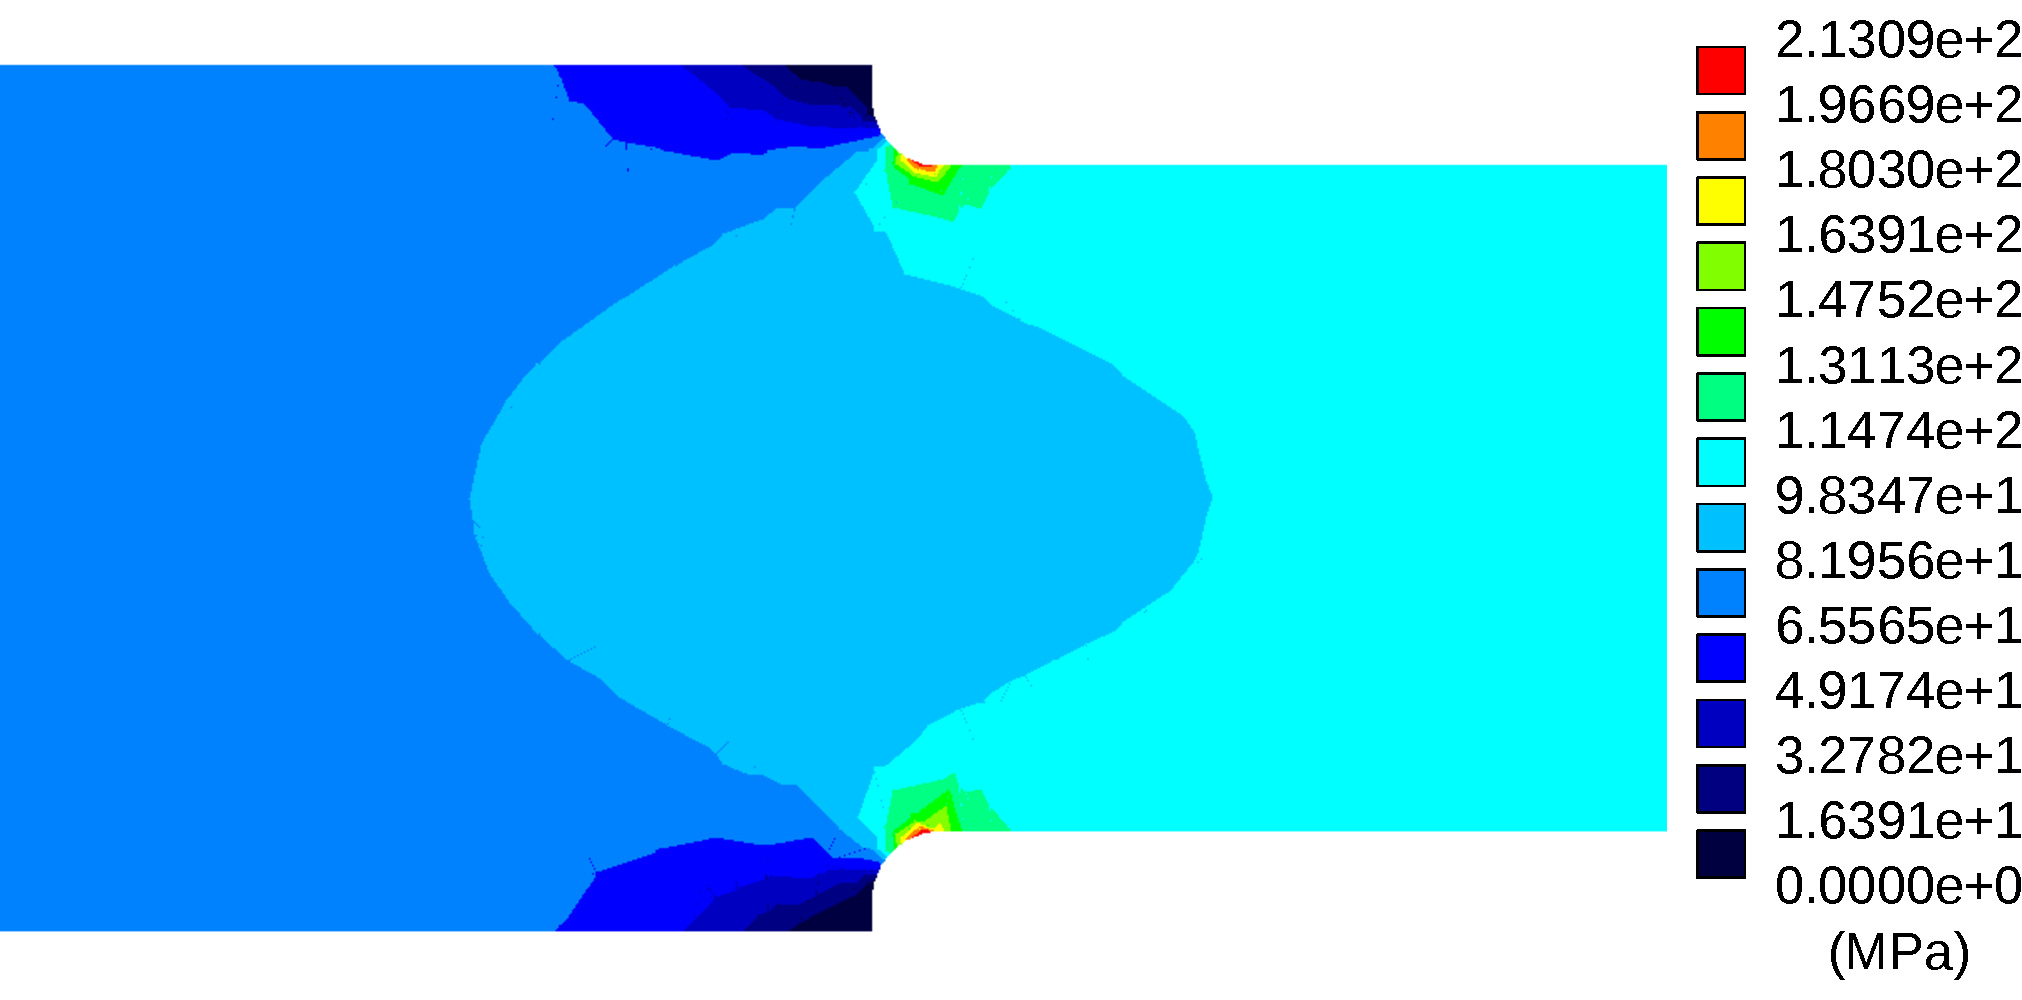
\includegraphics[width=\textwidth]{img/Hd1-3_rd0-10.pdf}
        \caption{$H/d = 1.3,r/d = 0.10$}
        \label{fig:H/d=1.3-r/d=0.10}
    \end{subfigure}
    \begin{subfigure}[b]{0.48\textwidth}
        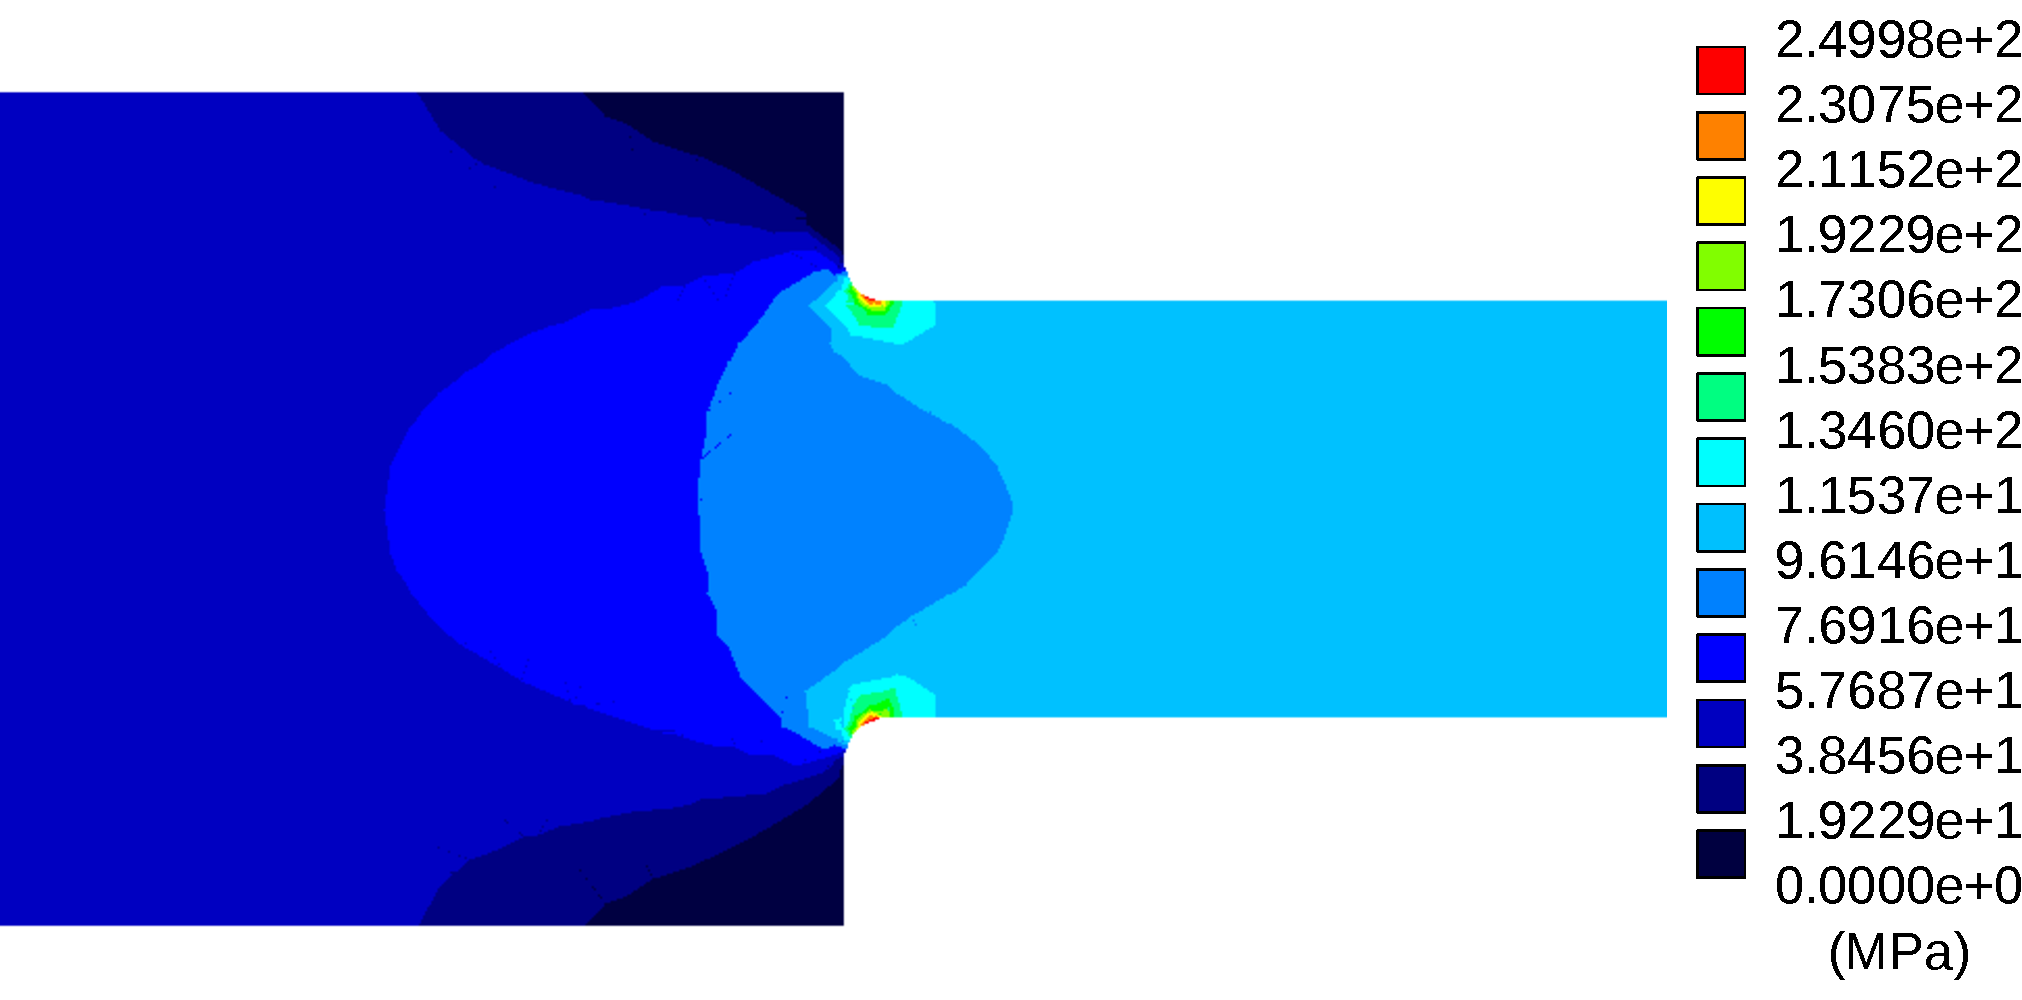
\includegraphics[width=\textwidth]{img/Hd2-0_rd0-10.pdf}
        \caption{$H/d = 2.0,r/d = 0.10$}
        \label{fig:H/d=2.0-r/d=0.10}
    \end{subfigure}
    \caption{Stress concentrations simulated for shoulder fillets with
        different $H/d$ and $r/d$.}
    \label{fig:simulation-results-contour}
\end{figure*}

The maximum stresses in each contour plot were divided by the far-field stress 
to find the stress concentration factor for each combination of $H/d$ and
$r/d$. These are recorded in Figure~\vref{fig:simulation-results-plot}, plotting
the stress concentration factor against $r/d$ for each $H/d$ on 
$\log_{10}$--$\log_{10}$ scale.

Least squares regression lines were fitted to the data in log-space, indicating
a power law relationship of the following form:
\begin{equation}
    K_{\sigma_t} = \alpha\left(\frac{r}{d}\right)^\beta
\end{equation}

\begin{figure}[H]
    \small
    \centering
    \def\svgwidth{\linewidth}
    \input{img/simulation_results.pdf_tex}
    \caption{Stress concentration factors of shoulder fillets with
        different $H/d$ and $r/d$. Scale: $\log_{10}$--$\log_{10}$}
    \label{fig:simulation-results-plot}
\end{figure}

Figure~\ref{fig:simulation-results-length} records the stress concentration
factor of shoulder fillets as the length of the plate was reduced from
effectively infinite to finite values.

\begin{figure}[H]
    \small
    \centering
    \def\svgwidth{\linewidth}
    \input{img/simulation_length.pdf_tex}
    \caption{Stress concentration factors of shoulder fillets with different
        $L/H$.}
    \label{fig:simulation-results-length}
\end{figure}

\section{Discussion}

\subsection{Circular Hole Stress Raiser}

Gauge 2 measured the nominal strain under axial load and gauge 1 is
perpendicular at the same location, suggesting the relationship between the
two strains can be described by the Poisson effect. Substituting
$\epsilon_{nom}$ and $\epsilon_1$ into \eqref{eq:poisson} yields the following:
\begin{equation*}
    \nu = -\frac{\epsilon_1}{\epsilon_{nom}} = -K_{\epsilon_1}
\end{equation*}

Therefore, Poisson's ratio for the plate used in the experiment can be obtained
from Table~\vref{tab:strain-conc}, which suggests a 95\% confidence interval
for $\nu$: $0.314\pm0.016$. Assuming the plate was made from machined aluminium,
a sensible alloy choice would have been 6086. According to the American Society
for Metals~\cite{asm1978metals}, Aluminium 6086 and similar alloys have a
Poisson's ratio of 0.33 at room temperature, which is contained in the 95\%
confidence interval for Poisson's ratio estimated empirically. At the 5\% level
of significance the measured Poisson's ratio did not differ from the true
Poisson's ratio of the material.

Gauges 5, 6, 7 and 9 were located on the plate boundary, so the axial load
form of Hooke's law applied. Substituting \eqref{eq:hooke-axial} into 
\eqref{eq:stress-conc} yields the expression for strain concentration factor 
given in \eqref{eq:strain-conc}:
\begin{equation} \label{eq:equiv-conc}
    K_\sigma = \frac{\sigma_{max}}{\sigma_{nom}}
             = \frac{\cancel{E}\epsilon_{max}}{\cancel{E}\epsilon_{nom}}
             = K_\epsilon
\end{equation}

From \eqref{eq:equiv-conc}, it can be deduced that the local stress
concentration factors at the locations of these gauges were the same as the
local strain concentration factors calculated in Table~\ref{tab:strain-conc}.
These are displayed in Table~\ref{tab:stress-conc}.

\begin{table}[h]
    \small
    \centering
    \caption{Local stress concentration factors measured around circular hole.}
    \label{tab:stress-conc}
    \begin{threeparttable}
        \begin{tabular}{
            c
            S[separate-uncertainty=true,
              table-format=-1.3,
              table-figures-uncertainty=1]
        }
            \toprule
            $K_{\sigma_5}$ &  1.001\pm0.033 \\
            $K_{\sigma_6}$ & -1.559\pm0.040 \\
            $K_{\sigma_7}$ &  4.564\pm0.103 \\
            $K_{\sigma_9}$ &  0.760\pm0.017 \\
            \bottomrule
        \end{tabular}
        \begin{tablenotes}
            \footnotesize   
            \item $K_{\sigma_i}\pm95\%$ confidence
        \end{tablenotes}
    \end{threeparttable}
\end{table}

Looking at the contour plot from the simulation in 
Figure~\ref{fig:experiment-simulation} reveals the maximum stress coincided
with the location of gauge 7. $K_{\sigma_7}$ is an empirical
measurement of the overall stress concentration factor in the plate.

\begin{figure}[h]
    \centering
    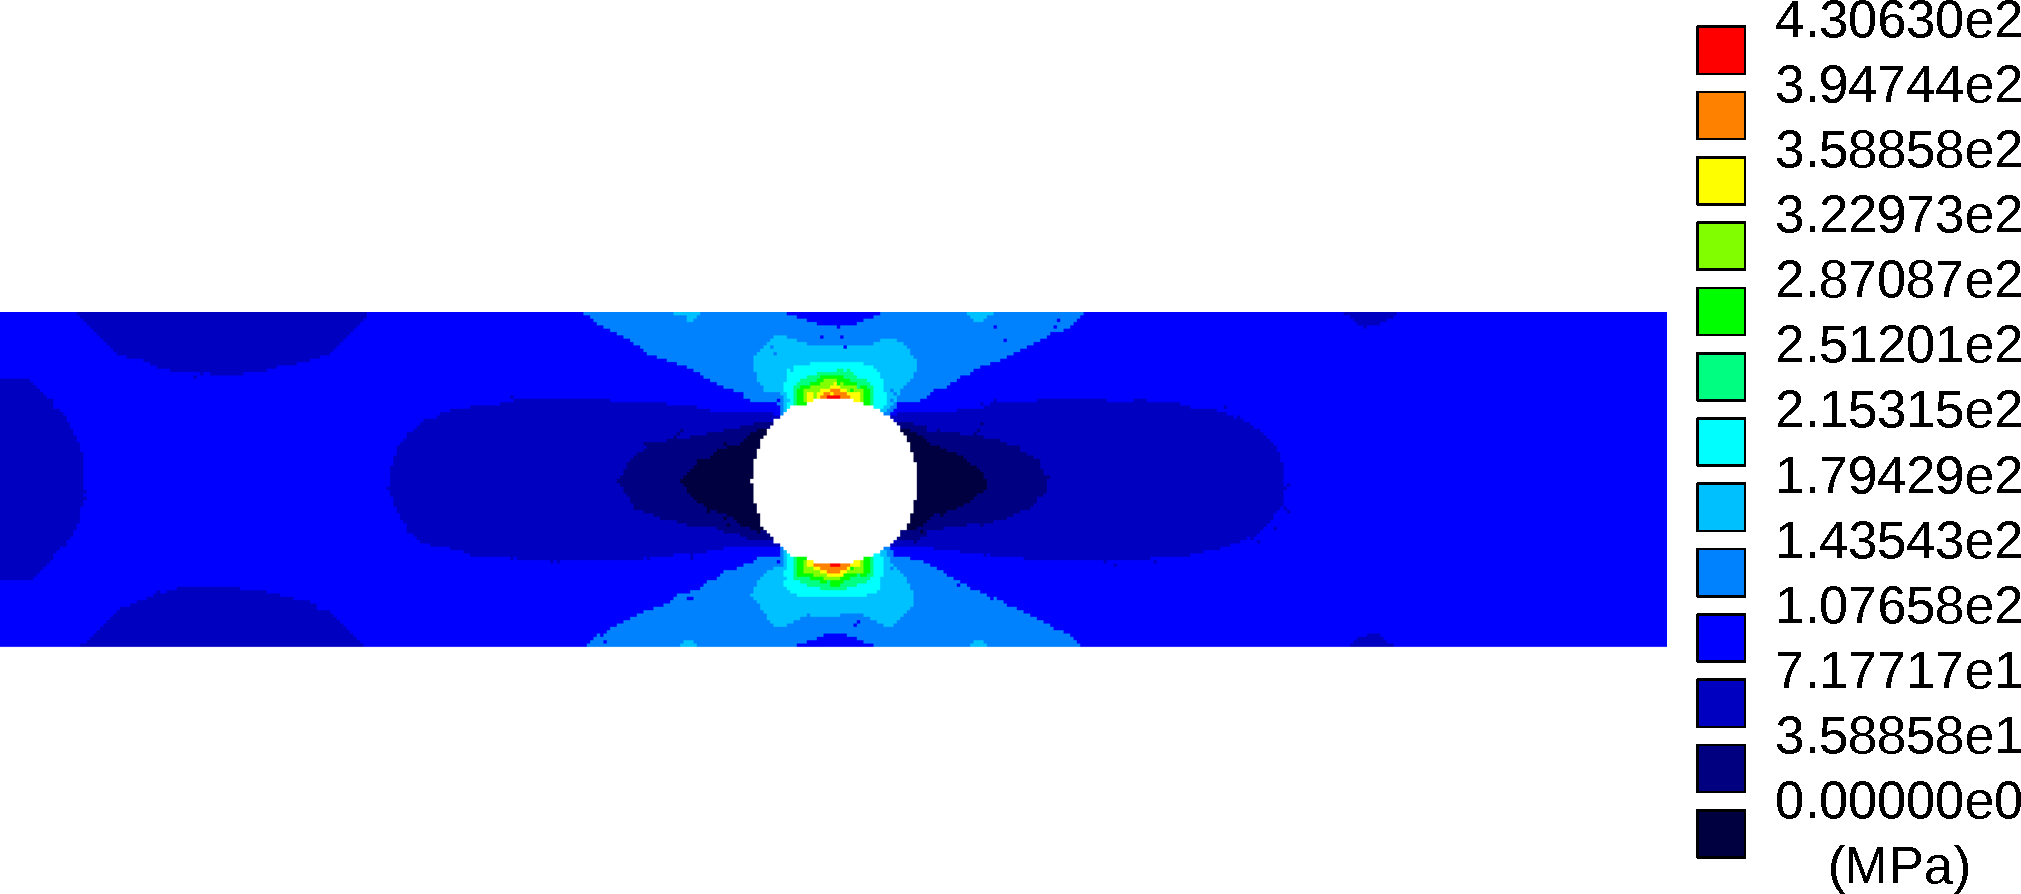
\includegraphics[width=\linewidth]{img/experiment_simulation.pdf}
    \caption{Stress concentrations simulated around circular hole.}
    \label{fig:experiment-simulation}
\end{figure}

The maximum stress recorded in Figure~\ref{fig:experiment-simulation} was
4.310~\MPa and the far-field stress applied was 100~\MPa. Applying 
\eqref{eq:stress-conc} yielded a numerical prediction of the stress
concentration factor. Another prediction was obtained by plugging the dimensions
of the plate in Figure~\ref{fig:experiment-dims} into the analytical equation,
\eqref{eq:hole-conc}. These are compared to the empirical value obtained in 
Table~\ref{tab:stress-conc-comparison}.

\begin{table}[h]
    \small
    \centering
    \caption{Comparison of approaches.}
    \label{tab:stress-conc-comparison}
    \begin{threeparttable}
        \begin{tabular}{
            l
            l
            S[separate-uncertainty=true,
              table-format=1.3,
              table-figures-uncertainty=1]
        }
            \toprule
            Analytical & $K_{\sigma_t}$ &    {4.250}    \\
            Numerical  & $K_{\sigma_t}$ &    {4.310}    \\
            Empirical  & $K_{\sigma_7}$ & 4.564\pm0.103 \\
            \bottomrule
        \end{tabular}
        \begin{tablenotes}
            \footnotesize   
            \item $K_{\sigma_7}\pm95\%$ confidence
        \end{tablenotes}
    \end{threeparttable}
\end{table}

The stress concentration factors predicted by \eqref{eq:hole-conc} and the
Concept Analyst simulation are similar to---but do not lie within---the 95\%
confidence interval for the stress concentration factor found empirically. At 
the 5\% level of significance, the stress concentration factor in the plate was
not what the theoretical values suggested after accounting for random errors.

It is unlikely the empirical value obtained was more accurate than prior
experiments which were the basis for the theoretical values above. The
systematic errors---or inaccuracies---in this experiment can be explained by
three main factors: inhomogeneity in the plate, calibration of the strain gauges
and different measurements of the far field stress.

Equation~\eqref{eq:hooke-axial}---Hooke's law under axial load---only applies
to members homogeneous in the axial direction. However, the plate may not have a
constant thickness, particularly at the machined edges. Although instructions
warn against tensioning the plate beyond \num{1000e-6} strain to avoid plastic
deformation, previous groups may have over-tensioned the plate. The most
stressed region at the location of gauge 7 would be the first to yield and
consequently the thinnest region. The thinnest regions are subjected a greater
stress concentrations which the analytical model and \BEM do not account for.
The argument also applies to the width of the plate.

Strain gauges increase in resistance as strain increases. The constant of
proportionality by which they change is calibrated upon installation, but over
time may vary due to temperature changes, break down of adhesives and
degradation of the strain sensitive resistor. If the constant of
proportionality for gauge 7 was greater than for gauge 2, the strain
concentration factor would be overestimated.

The nominal strain gauge 2 was located half way between the hole and the
boundary where the far field stress was applied. The contour plot in
Figure~\ref{fig:experiment-simulation} suggests this would lead to an
underestimation of the far-field stress, as stresses get smaller in the middle
of the plate close to the stress raiser. Equation \eqref{eq:strain-conc}
suggests $K_{\epsilon}$ and $\epsilon_{nom}$ are inversely proportional, so an
underestimation in far-field strain would lead to an overestimation in the
strain and stress concentration factors.

In practice, the factor of safety used to design parts can be increased to
account for the error in predictions of stress concentration factors.

\subsection{Shoulder Fillet Stress Raiser}

The contour plots in Figure~\vref{fig:simulation-results-contour} reveal the
most stressed regions of the shoulder fillets and the points of failure in
the event of yield were on the fillet radii close to where the boundary and the
far-field were tangential, for all ratios $H/d$ and $r/d$. This is consistent
with the most stressed regions of the circular hole stress raiser, detailed in 
Figures~\ref{fig:hole-contour} and \ref{fig:experiment-simulation}, which were
located on the top and bottom of the hole where the far-field was tangential to
the boundary.

In both cases these were the points where the force lines navigating the stress
raiser were most deflected and consequently most concentrated.

Conversely, the sharp corner on the outside of the feature radii experienced
zero stress. This is justified because there is no continuous path for the
force lines into and out of the the corner, so the corner bears neither load
nor stress.

The stress concentration factor decreased as the ratio of feature radius to
minor plate width---$r/d$---increased, according to an inverse power law.
This is evidenced by the negative gradient of the best fit lines in 
Figure~\ref{fig:simulation-results-plot}. 
Table~\ref{tab:simulation-results-model} lists coefficients of the power model
with which the lines were fitted.

\begin{table}[h]
    \small
    \centering
    \caption{Fitted power models for shoulder fillets plotted on
        Figure~\ref{fig:simulation-results-plot}. of the form 
        \mbox{$K_{\sigma_t} = \alpha(r/d)^\beta$}}
    \label{tab:simulation-results-model}
    \begin{threeparttable}
        \begin{tabular}{
            S[table-format=1.1]
            S[separate-uncertainty=true,
              table-format=1.3,
              table-figures-uncertainty=1]
            S[separate-uncertainty=true,
              table-format=-1.4,
              table-figures-uncertainty=1]
            S[table-format=1.5]
        }
            \toprule
            {$H/d$} & $\alpha$ & $\beta$ & {$R^2$} \\
            \cmidrule(lr){1-1}\cmidrule(lr){2-3}\cmidrule(lr){4-4}
            1.1\tnote{$\dagger$} 
                & 1.000\pm0.000  &    {$-0.2424$}   & {---} \\
            1.3 & 1.051\pm0.013  & -0.3065\pm0.0046 & 0.99988 \\
            2.0 & 1.062\pm0.014  & -0.3711\pm0.0052 & 0.99990 \\
            \bottomrule
        \end{tabular}
        \begin{tablenotes}
            \footnotesize
            \item[$\dagger$] Insufficient data to effectively determine 
                model.
            \item $\alpha,\beta\pm95\%$ confidence
        \end{tablenotes}
    \end{threeparttable}
\end{table}

From inspecting the closeness of the data to the model, and noting how near the
coefficients of determinability are to one, it can be deduced the models were a
good fit to the data when $H/d$ was 1.3 or 2.0. Formally, the overall $p$-values
from the minimised $\chi^2$ regression test statistic were \num{1.76e-7} and
\num{2.18e-7} respectively; at the 5\% significance level, the data was
consistent with the model. With only a single data-point, it was impossible to
determine whether data fitted any model when $H/d$ was 1.1.

The $\beta$ coefficients in the range $-0.4$ to $-0.3$, suggested increasing the
radius had less of an effect on the stress concentration factor as the magnitude
of radius increased, leading to diminishing reductions in stress concentrations.
However the range of the the ratio $r/d$ is bounded between zero and the height
of the step from the minor plate width $L$ to the major plate width $H$ as
follows:
\begin{align}
    \nonumber
    &\left\{
    \begin{aligned}
        r &> 0 \\
        H &\geq d + 2 r
    \end{aligned}
    \right. \\
    \Rightarrow
    &\;0 < \frac{r}{d} \leq \frac{1}{2}\left(\frac{H}{d} - 1\right)
\end{align}

Therefore, assuming the power law continues to hold, there exists a minimum
stress concentration factor in plate when the radius is at a maximum---the
distance from the major plate width to the minor plate width. In 
Figure~\ref{fig:simulation-extrapolated}, the lines in
Figure~\vref{fig:simulation-results-plot} have been extrapolated in linear-space
to the limits of $r/d$ to demonstrate this.

\begin{figure}[h]
    \small
    \centering
    \def\svgwidth{\linewidth}
    \input{img/simulation_extrapolated.pdf_tex}
    \caption{Extrapolated stress concentration factors of shoulder fillets for
        different $r/d$ and $H/d$.}
    \label{fig:simulation-extrapolated}
\end{figure}

Figure~\ref{fig:simulation-extrapolated} also illustrates the stress 
concentration factor becomes unbounded as the radius goes to zero. In practice,
its impossible to manufacture an shoulder without a small radius. Nonetheless,
including a radius feature in the design of shoulder features is critical to
avoiding large stress concentrations.

With regards to the change in plate width across the stress raiser, the effect
of increasing $H/d$ can be seen too. The plates with a greater ratio $H/d$ had
greater stress concentration factors for the same $r/d$ values. Consequently,
to maintain the same stress concentration factor for a greater $H/d$
ratio requires using a larger radius for the shoulder fillet.

In industry, engineers use more complete charts of a similar form to the one in
Figure~\ref{fig:simulation-extrapolated} to specify the geometry of the part
they are designing. It is more likely the ratio $H/d$ would be driving the
dimension of a shoulder fillet feature---on a shaft with a change in diameter
for example. The radius can then be specified to meet the stress concentration
factor requirement after considering the loads and failure criteria of the
material. An example of such a chart is referenced in
Section~\ref{sec:stress-conc} and referenced again 
\mbox{here~\cite[p.~151]{pilkey2008peterson}}.

These charts are only valid when the plate is sufficiently long with respect to
it's width. The plate in Figure~\vref{fig:H/d=2.0-r/d=0.10} was modelled with
$H/d$ at 2.0, $r/d$ at 0.10, $L/d$ at 10 and yielded a stress concentration
factor of 2.4998.

Figure~\ref{fig:simulation-results-length} indicates the stress concentration
factor remained largely constant when \mbox{$L/H > 3$}, accounting for numerical
noise. When \mbox{$L/H > 3$}, the mean for $K_{\sigma_t}$ was 2.4994 with a
one-tailed 95\% lower confidence limit of 2.4992, derived using the standard
error for $K_{\sigma_t}$ including data when $L/H$ was 6, 7, 8, 9 and 10.
Table~\vref{tab:simulation-results-length} lists the confidence limits for all
values tested and confirms 3 was the largest $L/H$ ratio for which the
reduction in stress concentration was significant at the 5\% level.

\begin{table}[h]
    \small
    \centering
    \caption{95\% confidence limits for mean $K_{\sigma_t}$ in shoulder fillets
        calculated from data when \mbox{$L/H > x$}, compared with $K_{\sigma_t}$
        measured when \mbox{$L/H = x$}.}
    \label{tab:simulation-results-length}
    \begin{threeparttable}
        \begin{tabular}{
            S[table-format=1.1]
            S[table-format=1.5]
            S[table-format=1.5]
            S[table-format=-1.2e-1]
        }
            \toprule
            \multicolumn{1}{c}{\multirow{2}{*}{\shortstack[c]{\\$L/H$}}} &
            \multicolumn{2}{c}{$K_{\sigma_t}$} &
            \multicolumn{1}{c}{\multirow{2}{*}{\shortstack[c]{
                $\text{Limit}$ \\$\text{}-\text{Actual}$
            }}} \\
            \cmidrule(lr){2-3}
            & {Limit\tnote{$\dagger$}} & {Actual} & \\
            \midrule
            0.5 & 2.47901 & 2.19150 &  2.88e-1 \\
            1.0 & 2.49247 & 2.41160 &  8.09e-2 \\
            1.5 & 2.49714 & 2.47130 &  2.58e-2 \\
            2.0 & 2.49881 & 2.49060 &  8.21e-3 \\
            2.5 & 2.49925 & 2.49720 &  2.05e-3 \\
            3.0 & 2.49925 & 2.49920 &  5.48e-5 \\
            \cmidrule(lr){1-4}
            3.5 & 2.49921 & 2.49960 & -3.86e-4 \\
            4.0 & 2.49916 & 2.49960 & -4.37e-4 \\
            4.5 & 2.49911 & 2.49940 & -2.87e-4 \\
            5.0 & 2.49903 & 2.49940 & -3.66e-4 \\
            % 6.0 & 2.49891 & 2.49930 & -3.85e-4 \\
            % 7.0 & 2.49861 & 2.49930 & -6.94e-4 \\
            % 8.0 & 2.49651 & 2.49940 & -2.89e-3 \\
            \bottomrule
        \end{tabular}
        \begin{tablenotes}
            \footnotesize
            \item[$\dagger$] $\text{mean}-\text{95\% confidence}$
        \end{tablenotes}
    \end{threeparttable}
\end{table}

Consequently, the model in Figure~\vref{fig:simulation-extrapolated} is not a
good fit when $L/H \leq 3$. Similar length constraints will apply for different
$H/d$ and $r/d$ ratios to the respective 2.0 and 0.10 values chosen for this
analysis.

\section{Conclusions}

For finite width plates with circular hole and shoulder fillet stress raisers,
the most stressed points both lie on the plate boundary at the top or bottom of
the hole or on the inside of the shoulder fillet, where the force lines through
the part are most concentrated.

Simulations can be used to find stress concentration factors which are close to
the true stress concentration factors in the material. However, small errors in
measurements can lead to lead to inaccuracies in predictions. This reaffirms the
importance of factors of safety in the design of structural parts.

Simulations outlined the relationship between shoulder fillet radii and stress
concentration factors in plates, suggesting an inverse power law. Extrapolating
the power law revealed small fillet radii lead to very large stress
concentration factors and the minimum stress concentration factor is achieved by
maximising the fillet radii.

The same simulations also suggested increasing the ratio of the major plate
width over the minor plate width leads to greater stress concentration factors
for the same fillet radii. Engineers can use charts and tables to specify the
required fillet radii for a particular part to meet loading requirements.

The models used and relationships derived in this report apply to plates of a
sufficient length. For plates with shoulder fillets, when the ratio of the
length over the width of plate is 3 or less, alternative models must be devised.

% References.
\printbibliography

\end{document}